In this chapter, we present experimental results of the LPNN approach. The evaluation is qualitative, since the nature of light probes and their optimal placement is subjective to the user and the needs of the application. We focus mainly on speed of execution in relation to light probe layout given by the tool. We compare performance results to LumiProbes \parencite{Vardis2021}. All experiments were conducted in Unity 6 version 6000.0.38f1, on a system comprising of an NVIDIA RTX2060M GPU, 16GB DDR4 RAM and an Intel i7-9750H CPU, on a Windows 10 Operating System.

\section{Performance}
\label{sec:4_performance}
Since the focus of the thesis was to speed up the placement of light probes in this stage of any 3D application development iteration process, we will focus on the execution time of the tool and also critique the results and their qualitative properties shortly, to make sure the placements are correct. Indeed, as seen in table \ref{table:times}, the LPNN approach speeds up light probe placement by orders of magnitude faster than the LumiProbes, but it may suffer from occasional misplacement; probes that were placed in positions that are not vital, leading to oversampling, which we will show shortly. 

In experiments where LumiProbes and LPNN were requested to place close to the same amount of light probes in the same scene, LPNN time stayed close to constant, typically up to a few seconds, regardless of the scenario or the amount requested. Results for various amounts of light probes and scenes are presented in table \ref{table:times}. Times are averaged over multiple runs. Units are represented in minutes (m), seconds (s), or milliseconds (ms). Where applicable, we also append the settings used for each tool. For LumiProbes, settings include the grid parameters and the evaluation-point count. All other settings are as follows: Evaluation point placement type is set to Poisson, Decimation type is set to Medium, Decimation directions are averaged, Decimation metric is set to  Chrominance, Minimum LP set is disabled, and Maximum Error is set to 3. For LPNN, settings include the threshold value used for the specific result and the cell size of the 3D grid, in order.\newline

Figures for the results are shown in section \ref{sec:4_quality}. Memory requirements for this tool are strictly dependent on the amount of light probes present in the scene, since all information needed by the tool is either already present in Unity and are needed regardless of the presence of the tool, e.g. Global Illumination data, or are stored on the Hard Disk of the system as files with storage sizes dependent on the amount of probes placed before the execution of the tool. File sizes for 150 probes were less than 2KB. Typically, the tool creates files needed for placing the light probes with size-scaling 1KB per approximately 100 probes.

\begin{table}
	\centering
\begin{tabular}{ |c||c|c|c|c|c|  }
	\hline
	\multicolumn{6}{|c|}{Execution Results} \\
	\hline
	Method & Scene & Time & P. Count & P. Present (\&Removed) & Settings\\
	\hline
	LumiProbes & Sponza   & 22.443s  & 105 & 34 (75)  & (7,3,5), 128 \\
			   &          & 600.285s & 240 & 54 (186) & (12,4,5), 256 \\
			   &          & $>$20000s & 420 & -----   & (14,5,6), 256 \\
	\cline{2-6}
	           & Office   & 51.059s  & 144 & 84 (60)  & (12,3,4), 128\\
	           &          & 919.134s & 288 & 182 (106)& (12,3,8), 256\\
	           &          & $>$20000s & 630 & -----   & (14,5,9), 256\\
	\cline{2-6}
	           & Corridor & 161.151s & 180 & 120 (60) & (20,3,3), 256\\
	           &          & 477.648s & 243 & 147 (96) & (27,3,3), 256\\
	\hline
	\hline
	Ours       & Sponza   & \textbf{5.3ms}  & 90  & 54 (36)   & 0.4, 2.0 \\
			   &          & \textbf{17.8ms} & 400 & 40 (360)  & 0.9, 1.3 \\
	\cline{2-6}
			   & Office   & \textbf{7.8ms}  & 140 & 34 (106)  & 0.758, 1.87 \\
               &          & \textbf{25.2ms} & 832 & 117 (715) & 0.859, 1.10 \\
    \cline{2-6}
    		   & Corridor & \textbf{10.9ms} & 186 & 84 (102)  & 0.549, 1.94 \\
               &          & \textbf{15.7ms} & 246 & 95 (151)  & 0.615, 1.50 \\
               
	\hline
\end{tabular}
\caption{Execution time for LPNN and LumiProbes on a select number of scenes and probe counts. \textit{P. count} represents the total amount of probes in the scene, before simplification. \textit{P. Present} depict the final amount of probes after running the tools. The number in parenthesis is the amount of probes removed by the tool, in respect to the settings. Fastest times are shown in \textbf{bold}.}
\label{table:times}
\end{table}

For execution times greater than 20000 seconds (approximately 5 hours and 30 minutes) the execution was forcibly stopped. Therefore, results for those occurrences are not collected, since for most scenarios and 3D scenes, the time needed for manual placement of light probes is shorter than 5 hours.

\section{Quality}
\label{sec:4_quality}

The tools were tested on the aforementioned edited Sponza scene \parencite{Sponza2017}, Corridor scene \parencite{Corridor2021} and Office scene \parencite{Office2021}. We will present the qualitative results. As we will see shortly, LPNN correctly places light probes in areas of high variance.

\subsection{Light Probe placement Quality}
\label{sec:lp_quality}

Before we can describe and analyze the layout provided by the tool, it is vital to describe what defines a high-quality light probe layout.

High-quality light probe placement optimally balances capturing lighting fidelity against the desired resource constraints. Light probes should be concentrated in regions where direct or indirect illumination exhibits rapid variation in space, such as near shadow edges, light occluders or areas with strong color bleeding. Placement of light probes in such locations is vital in order to minimize interpolation error of the irradiance information. Conversely, uniformly lit areas, such us open environments, probe density can be reduced to a minimum without perceptible loss of quality.

As seen in figure \ref{fig:transition_comparison} and figure \ref{fig:transition_comparison_lp}, the light probe layout depends highly on the surrounding context of the scene. By adapting probe density to lighting variance and geometric complexity, we ensure that the global illumination information received by dynamic objects in the scene is sufficient to reconstruct a close approximation of the true ground-truth solution, being path-tracing as mentioned in section \ref{sec:offline}, while placing the fewest probes possible depending on the resource limits.

\begin{figure}[h]
	\centering
	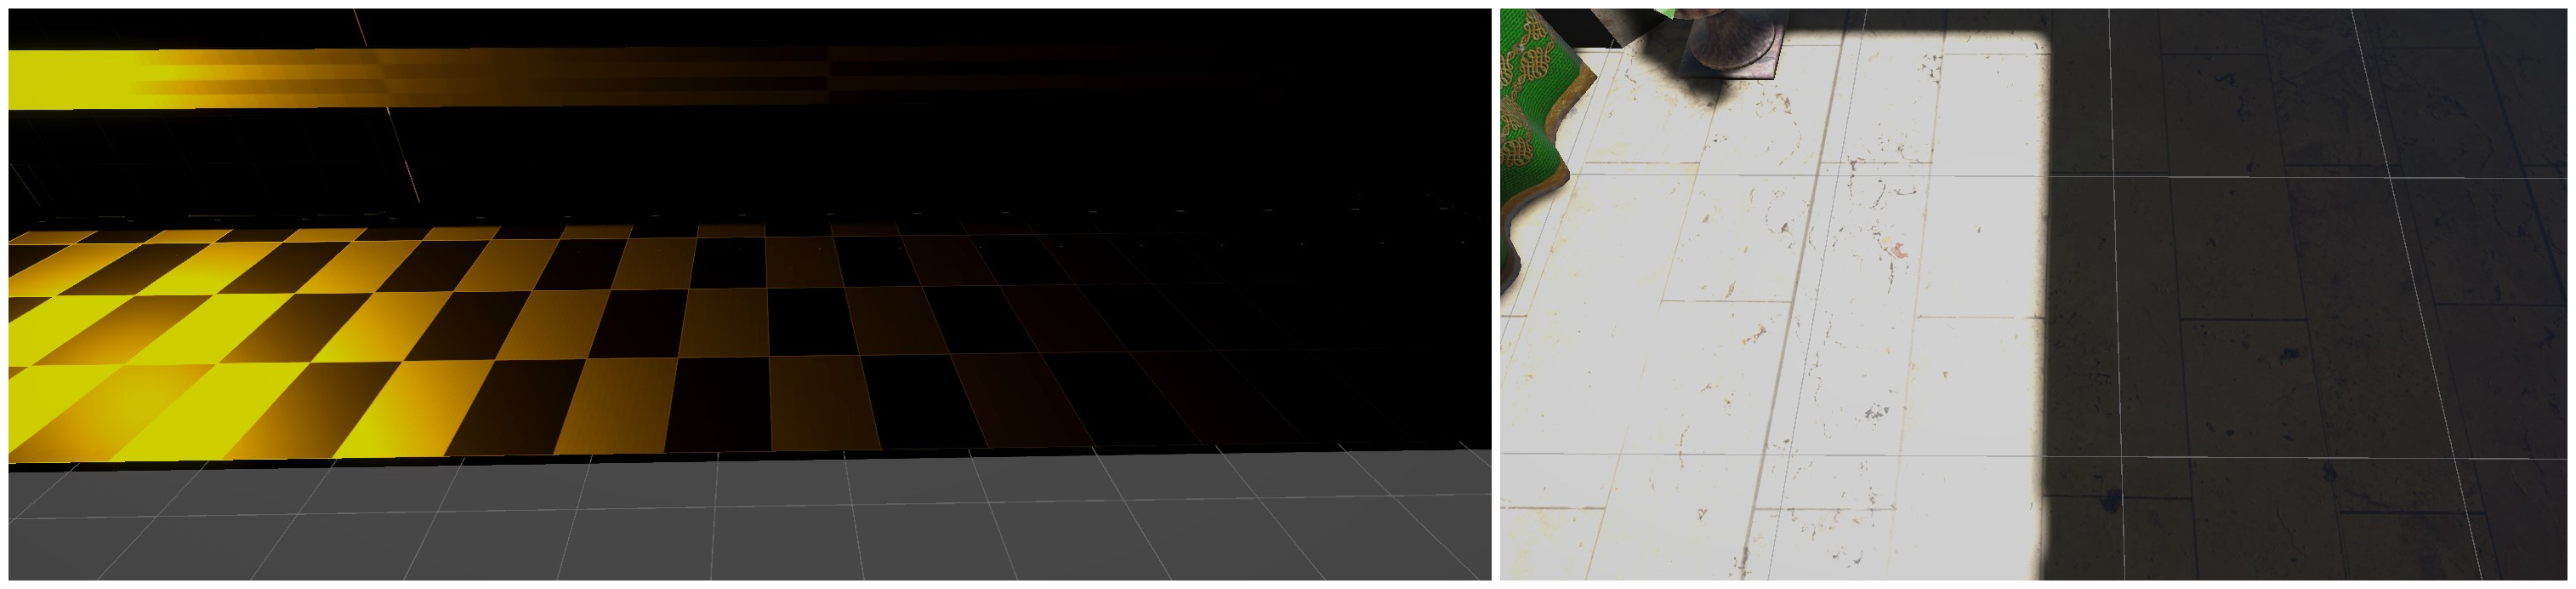
\includegraphics[width=\linewidth]{Graphics/results/concats/comparison7.png}
	\caption{Comparison between a location of gradual transition of the illumination, compared to a more instantaneous change. Examples taken from Corridor scene (left) and Sponza scene (right).}
	\label{fig:transition_comparison}
\end{figure}

A lower amount of light probes avoids long light baking times as well as reducing memory requirements in runtime. Additionally, if the probes are placed manually, a smaller amount of light probes makes the manual layout a process taking a fraction of the time required by a larger count. This enables artists to iterate rapidly, both in cases of manual placement and automatic placement tools, like the one proposed in this thesis.

\begin{figure}[h]
	\centering
	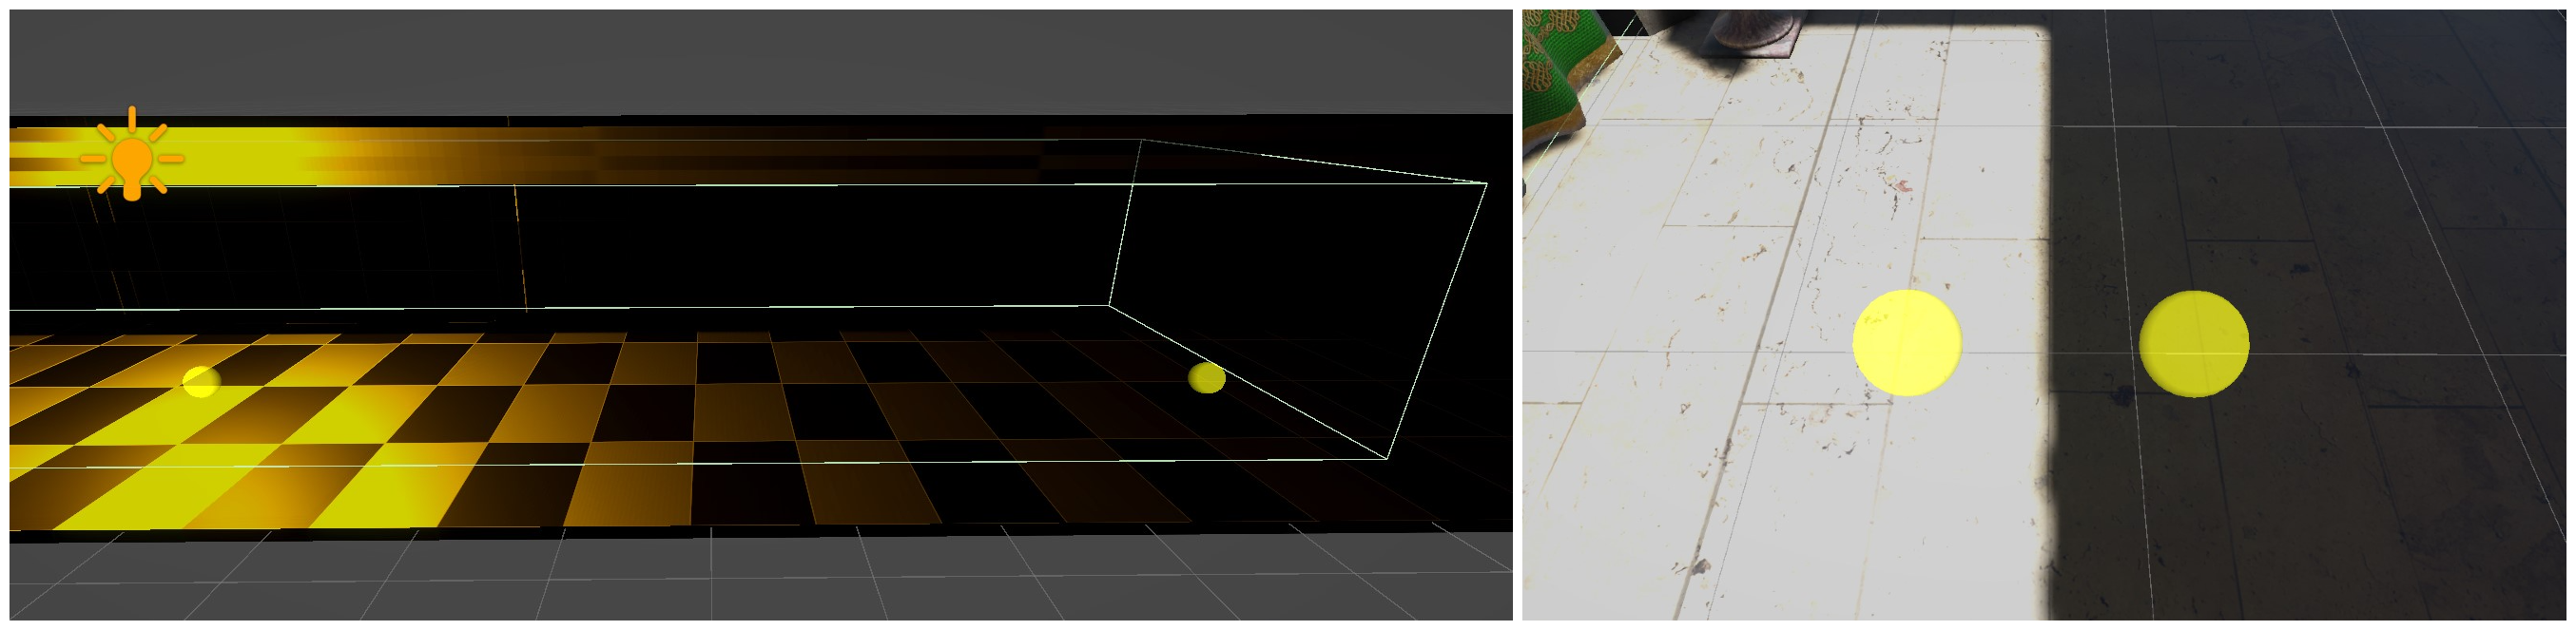
\includegraphics[width=\linewidth]{Graphics/results/concats/comparison8.png}
	\caption{Scenes depicting locations of close-to-optimal light probe placement, depending on the context of the scene and the location currently shown. Worth noting is the fact that the amount of light probes depicted is not enough to created a working light probe group inside Unity, which requires four or more light probes to create a tetrahedron. The layout depicted is only for clarity reasons, and not application-ready. Examples taken from Corridor scene (left) and Sponza scene (right).}
	\label{fig:transition_comparison_lp}
\end{figure}

Equally important to the density of the probes is maintaining spatial uniformity and coverage of the scene. Light probes must be far apart enough that the developer avoids wasting memory and reduces bake time, but clustered enough that no interpolation errors are present; errors that produce visible seams in the lighting as objects move between the tetrahedral cells of the probes. A high-quality placement strategy enforces a range of ideal distance between light probes to avoid gaps or clusters.

\subsection{Indoors Example}

\begin{figure}[h]
	\centering
	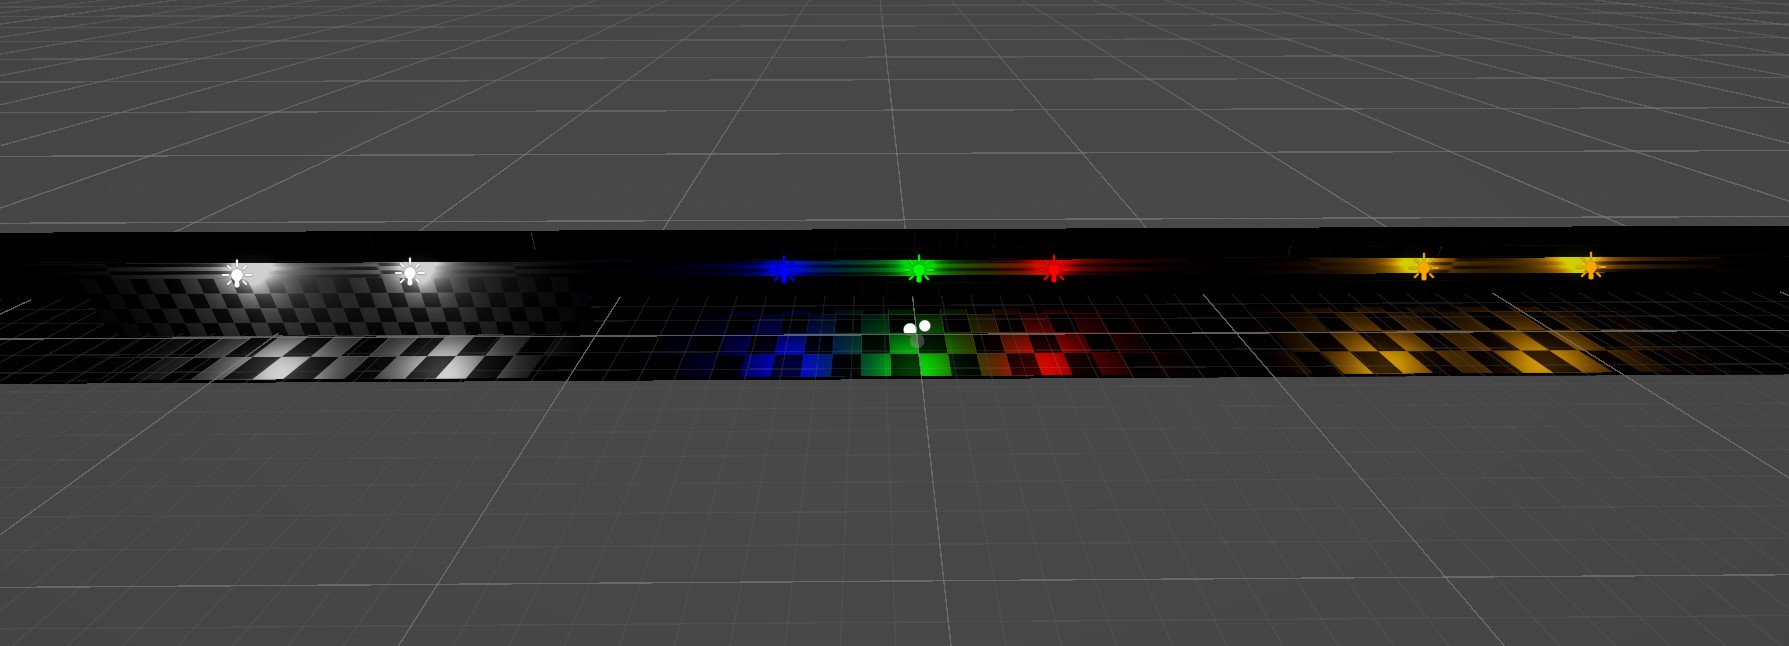
\includegraphics[width=\linewidth]{Graphics/results/corridor.jpg}
	\caption{The Corridor scene \parencite{Corridor2021} without any light probes placed. We show only the area of the scene that is inside the bounds of both LPNN and LumiProbes tools.}
	\label{fig:corridor}
\end{figure}

As shown in figure \ref{fig:comp1}, we can clearly see that the LPNN tool has correctly placed light probes between the blue and green light sources, as well as between the green and red light sources, locations with great variance in Chrominance, It has additionally kept the amount of probes at a minimum, only placing one probe at each location mentioned. This result is close to optimal placement, since the distance between the light sources is only 4 units, making additional probes unnecessary in most scenarios. It should be noted that the tool did correctly place probes on the edges of the bounds, seen as light-green colored lines. This ensures that any dynamic object that moves outside the bounds set by the user continues to have some light-probes information for its illumination. 

\begin{figure}[h]
	\centering
	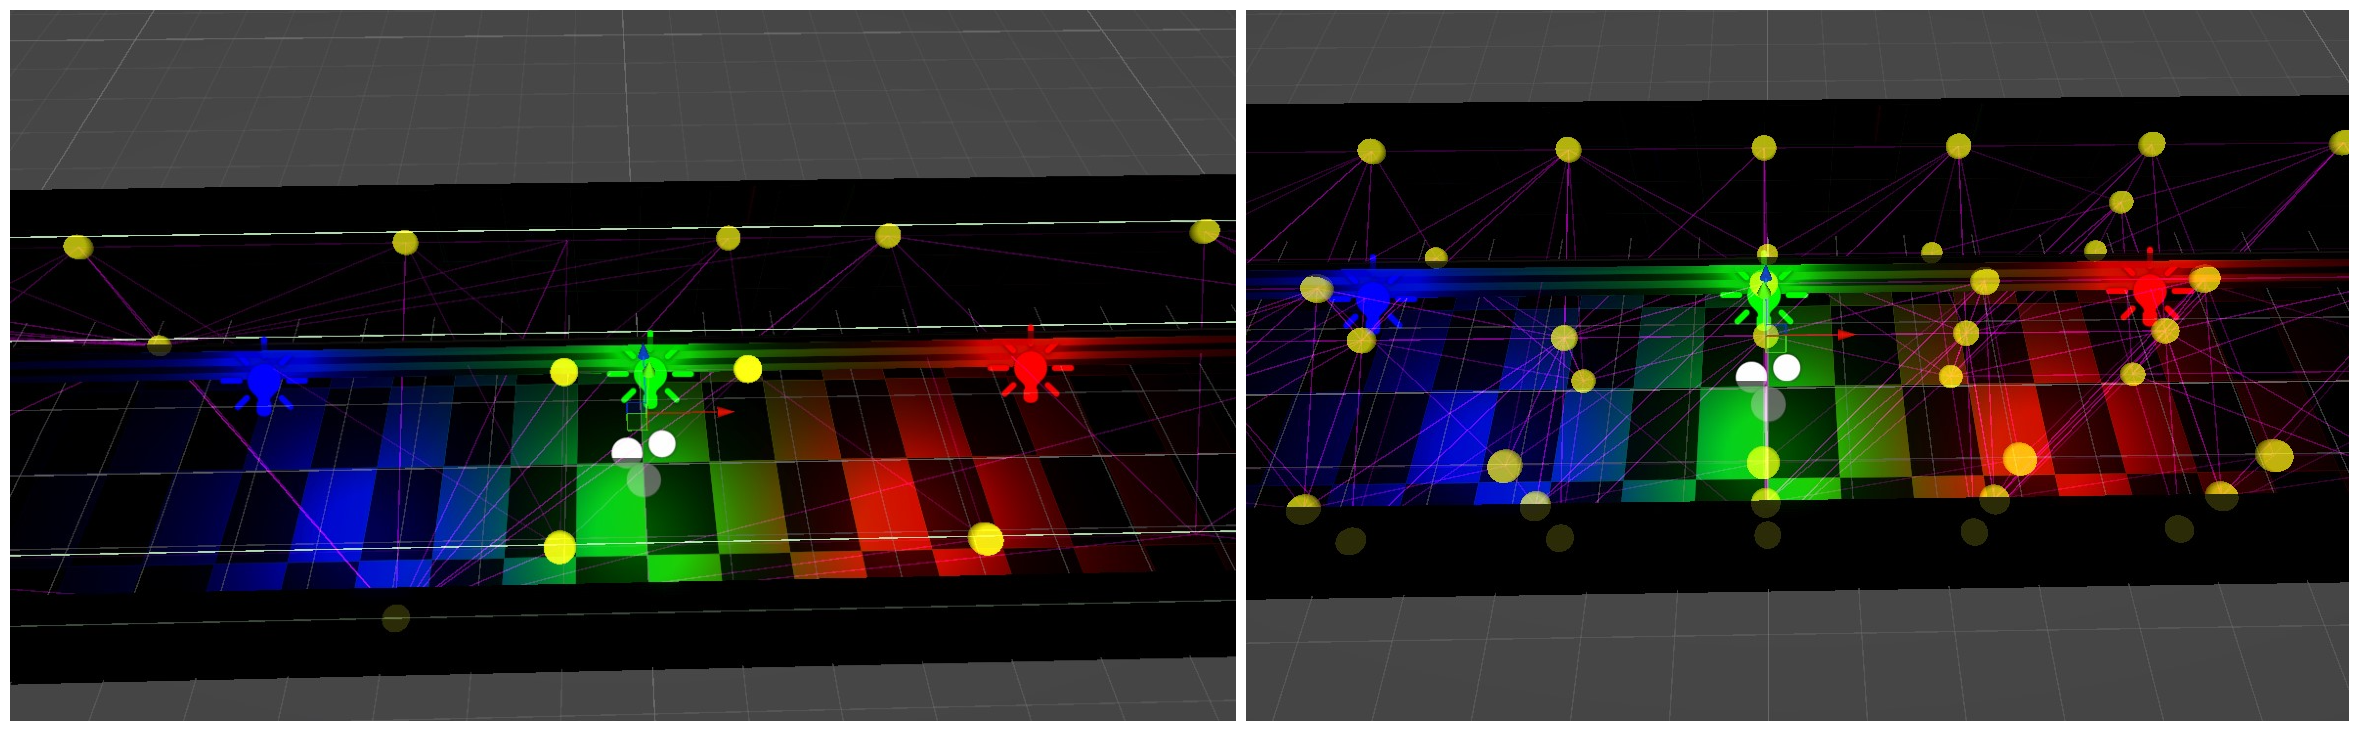
\includegraphics[width=\linewidth]{Graphics/results/concats/comparison1.png}
	\caption{An indoor 3D Scene showing a comparison of light probe placement in a \textbf{high} color-variance scenario, between LPNN (left) and LumiProbes (right) with settings 0.549, 1.94 and (27,3,3), 256 respectively, in the Corridor scene.}
	\label{fig:comp1}
\end{figure}

Furthermore, in figure \ref{fig:comp2} we can see a similar result. The light probe between the two white light sources is vital. The areas left and right from the two light sources have light probes only in the dark areas, making the light transition when a dynamic object moves within this section of the scene smooth. Additionally, the light sources are next to an opaque wall, meaning no light present on the other side of the wall. Therefore, the model decided that placing light probes is only important on the edges of the wall, which is what we see in the example. It is important to note that on the left side of the corridor, as seen in the left image of figure \ref{fig:comp2}, the model has placed a great amount of light probes, even though there is low light variance since that section of the scene is not illuminated. 

\begin{figure}[h]
	\centering
	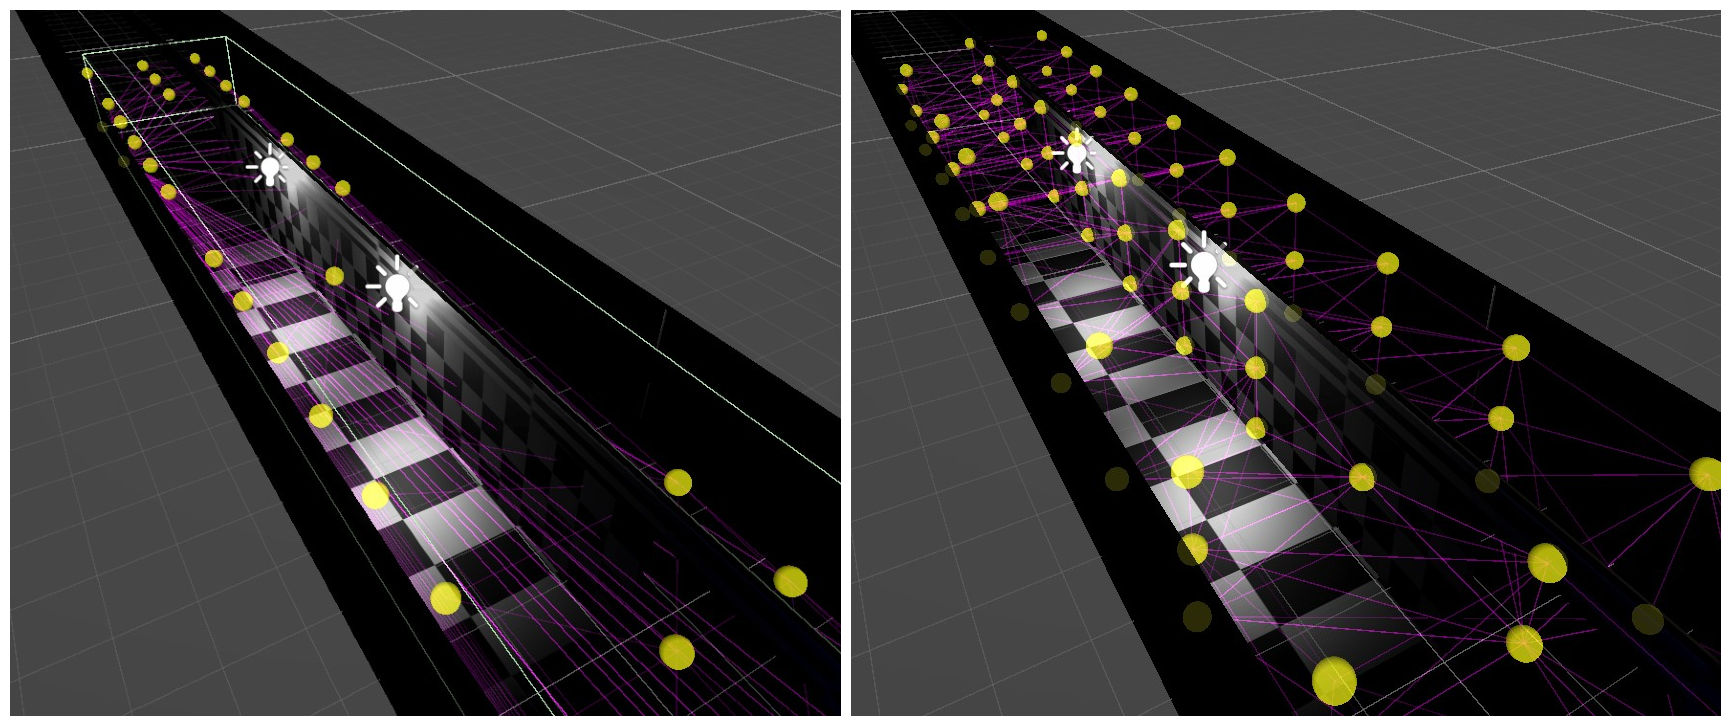
\includegraphics[width=\linewidth]{Graphics/results/concats/comparison2.png}
	\caption{A 3D Scene showing a comparison of light probe placement in a \textbf{low} color-variance scenario, but \textbf{high} luminance variance, between LPNN (left) and LumiProbes (right) with settings 0.615, 1.5 and (27,3,3), 256 respectively, in the Corridor scene.}
	\label{fig:comp2}
\end{figure}

Additionally, as seen in figure \ref{fig:comp3}, the model suffers from under-sampling in certain scenarios; placing fewer light probes than necessary, resulting in partially incorrect lighting. However, this can be resolved in two immediate ways; the user can execute the tool again with different parameters, as seen in figure \ref{fig:comp4}, or the user can manually place a small number of light probes in locations they deem vital. The tool has placed only 2 light probes on the lower section of the scene, resulting in elongated tetrahedrons and incorrect lighting for dynamic objects placed low. Additionally, the light probes placed on the dark side of the wall in figure \ref{fig:comp3} require one more row of light probes placed next to the wall, making any object inside that section of the scene completely dark due to the lack of light in that section. With the settings present in figures \ref{fig:comp1}, \ref{fig:comp2}, and \ref{fig:comp3}, the tool doesn't have enough light probes in the desired locations to correct this issue. This can be fixed by decreasing the cell size parameter, as seen in figure \ref{fig:corr_1}.

With better grid layout, the model correctly placed probes on both sides of the wall, correctly capturing the lighting information of the area. This can be seen in figure \ref{fig:corr_1}. On the left side of the wall, a number of probes were placed around the light sources, making any dynamic object that traverses the location have accurate illumination data. Similarly, on the right side of the wall, we can see probes placed flush with the wall, capturing the lack of light of the area, regardless of the proximity to light sources. This ensures that a dynamic object will remain unlit from the two light sources, if it is placed on the right side of the wall. 

\begin{figure}[h]
	\centering
	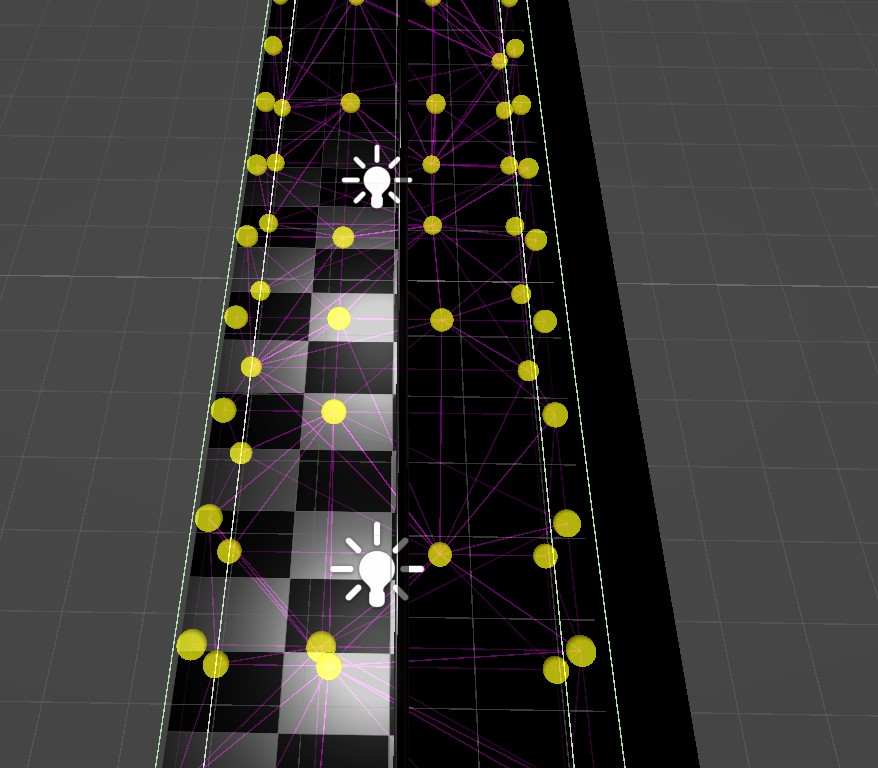
\includegraphics[scale=0.4]{Graphics/results/corridor_0.244_1.3.jpg}
	\caption{A 3D Scene showing a better placement of light probes in the Corridor scene, fixing the under-sampling issue of figure \ref{fig:comp2}. The example was captured with LPNN with settings 0.244, 1.3.}
	\label{fig:corr_1}
\end{figure}

It is worth noting that the model inferred that more points between the two light sources are important, placing three instead of one in figure \ref{fig:comp2}. Even though this can be considered as slight oversampling, the amount of additional light probes is minimal.

This result can be recreated for figures \ref{fig:comp1} and \ref{fig:comp3} with the same steps as before; a decrease in the cell size for better sampling, with a finer-tuned threshold value. This will result in light probes being placed flush with the beam present on the top of the scene, or any other under-sampling scenario.

\begin{figure}[h]
	\centering
	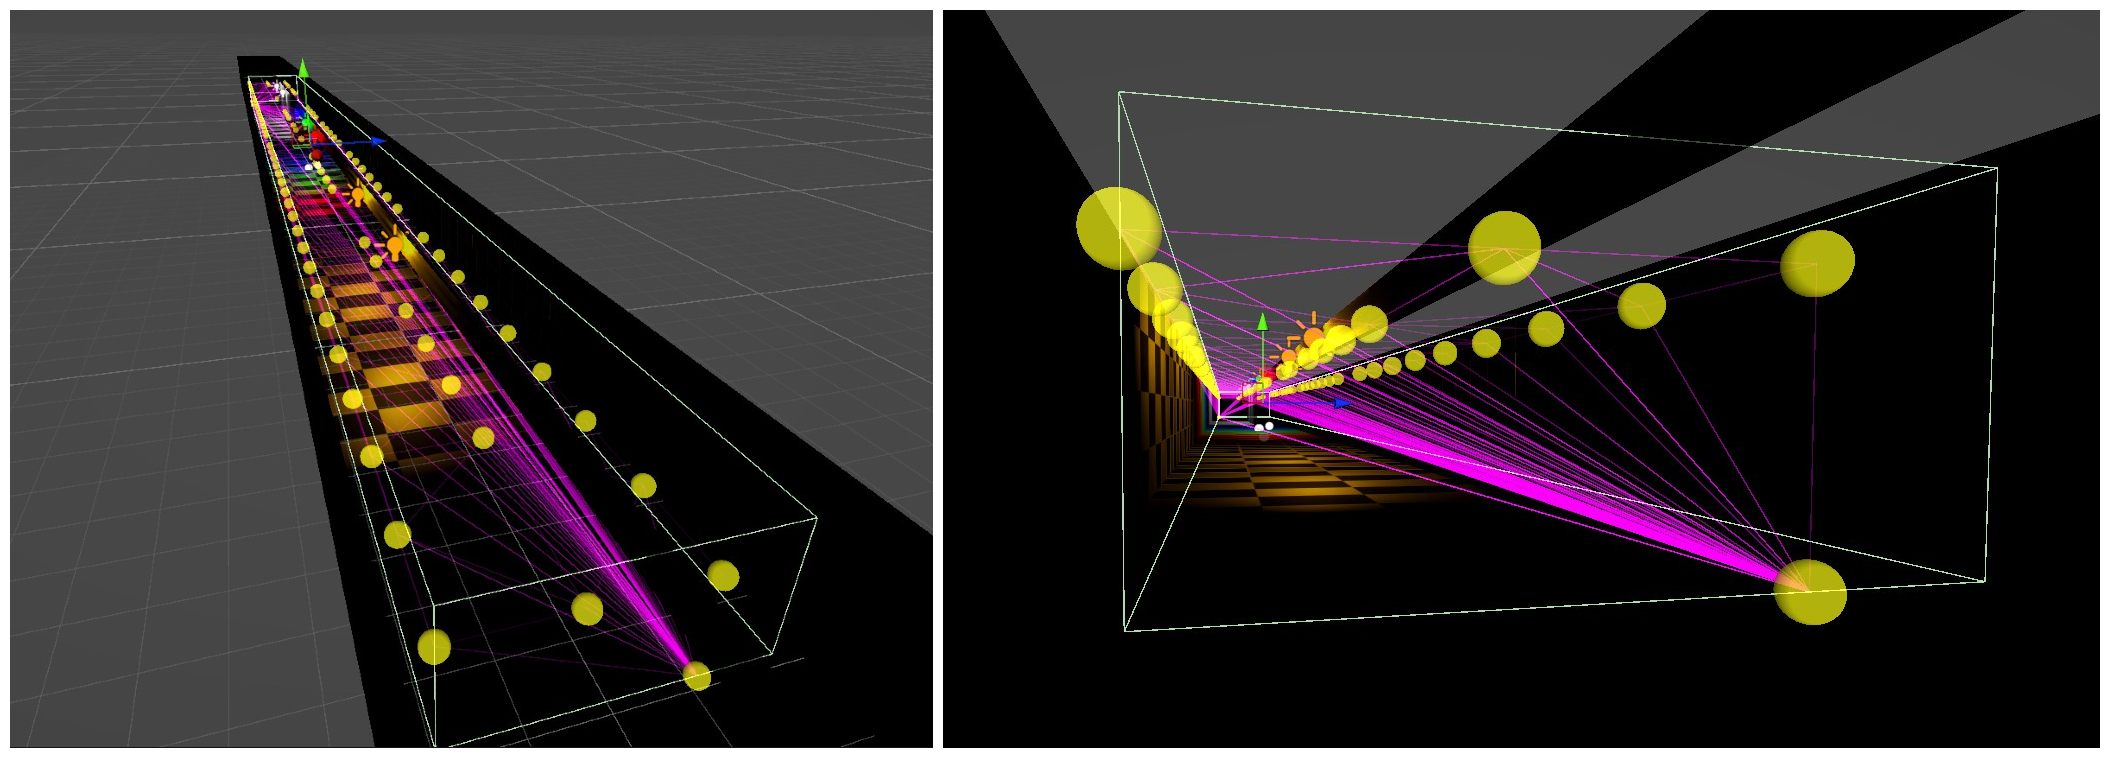
\includegraphics[width=\linewidth]{Graphics/results/concats/comparison3.png}
	\caption{A 3D Scene showing under-sampling of light probe placement in the Corridor scene. The example was captured with LPNN with settings 0.615, 1.5.}
	\label{fig:comp3}
\end{figure}

As mentioned, with different settings, we can resolve the under-sampling issue from figure \ref{fig:comp3}, as seen in figure \ref{fig:comp4}. By increasing the cell size but reducing the threshold, the tool has placed more probes on the lower section of the scene, from just 2 to 8, leading to better results overall. This can be further increased with additional tuning of the settings, but it may lead to oversampling in certain high-variance locations elsewhere in the scene.

\begin{figure}[h]
	\centering
	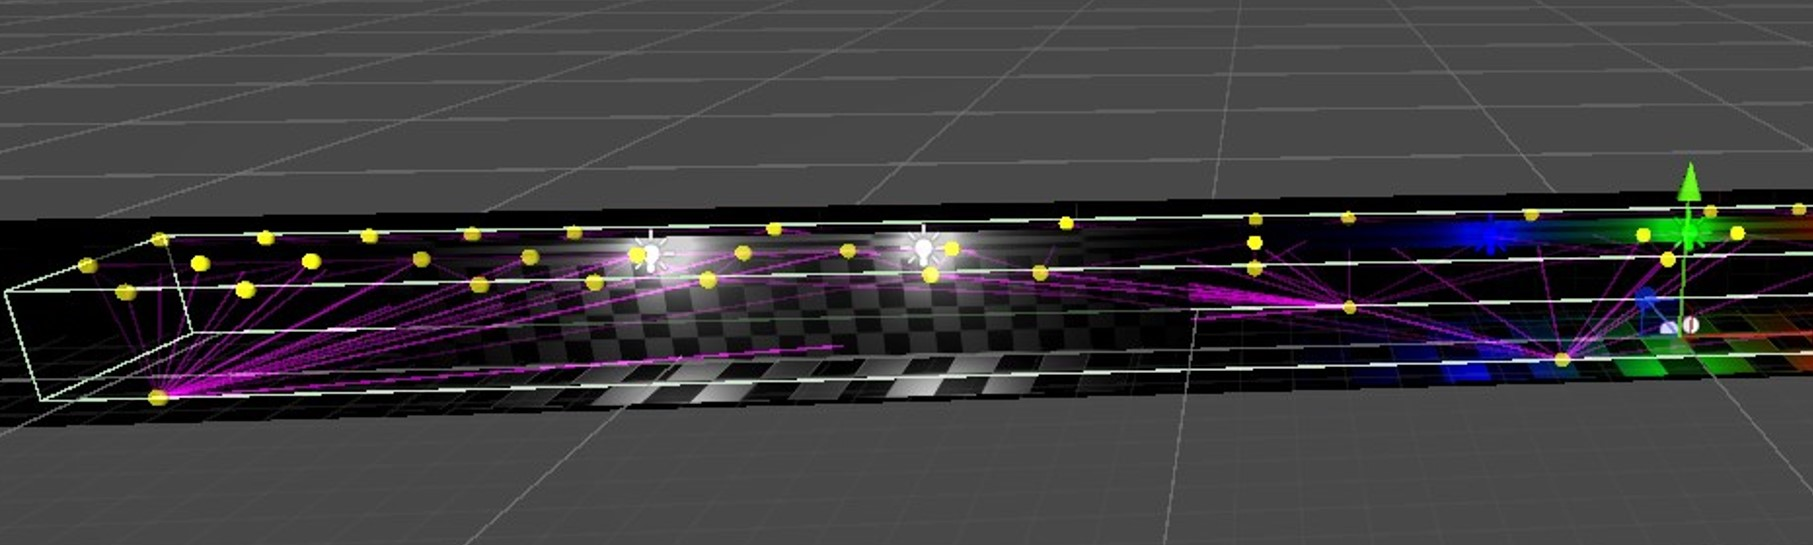
\includegraphics[width=\linewidth]{Graphics/results/corridor_0.549_1.94_E2.jpg}
	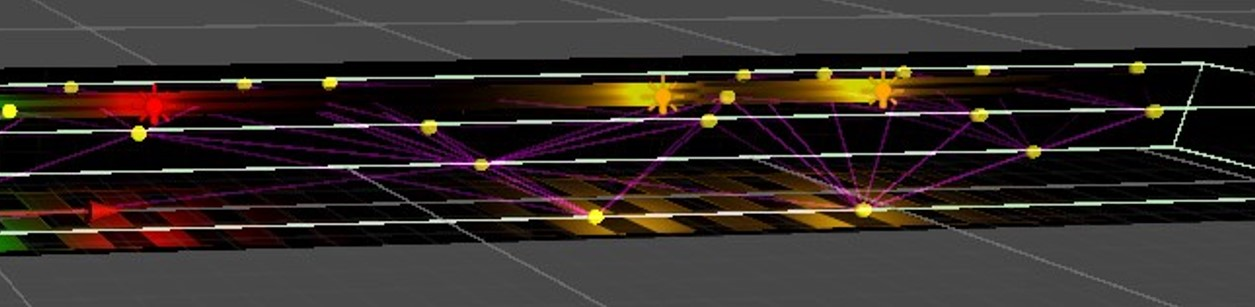
\includegraphics[width=\linewidth]{Graphics/results/corridor_0.549_1.94_E3.jpg}
	\caption{A 3D Scene showing improved light probe placement in the Corridor scene. The example was captured with LPNN with settings 0.549, 1.94.}
	\label{fig:comp4}
\end{figure}


\subsection{Outdoors Example}
\label{sec:outdoors}

So far, only results of indoors scenes have been shown and described. Indoor scenes are ones where all the illumination provided by the light sources, (lamps or the outdoor light leaking through the windows of a room) is contained within an area bounded by opaque surfaces like walls. However, in addition to indoor scenes, outdoor scenes are equally as important in a lot of 3D applications. The Sponza scene \parencite{Sponza2017} is an outdoors environment, where illumination is provided by a light source closely imitating a sun. The presence of walls without a ceiling, together with the sun angle being not-vertical to the floor, leads to interesting shadows and light interactions within the objects. As we will see shortly, LPNN speeds up the process of placing light probes in the scene significantly, requiring only minimal manual tweaking.

\begin{figure}[h]
	\centering
	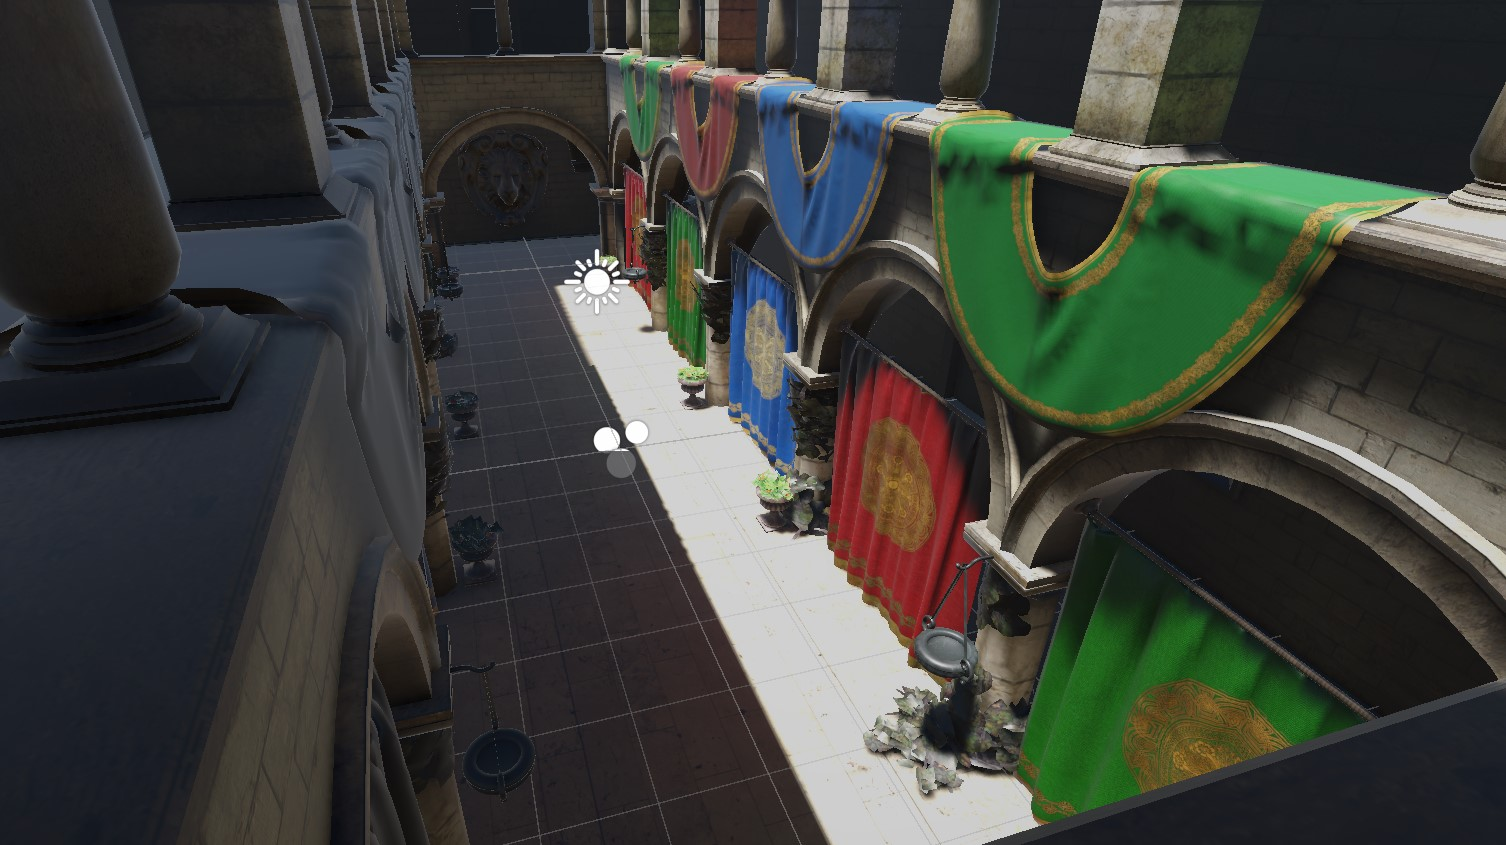
\includegraphics[width=\linewidth]{Graphics/results/sponza.jpg}
	\caption{The Sponza scene \parencite{Sponza2017} without any light probes placed. We show only the area of high importance, where the light probes should be placed.}
	\label{fig:sponza}
\end{figure}

Seen in figure \ref{fig:comp5}, the LumiProbes tool has placed several light probes on the two sides of the shadow created by the angled sun direction. This ensures that a dynamic object traversing the floor of the scene will receive GI information from the light probes, making the transition between the illuminated side on the right and the shadowed side on the left smooth. 

At first glance, the layout proposed by the LPNN tool for the settings mentioned in the caption of the figure, seems incorrect. The edge between the illuminated and the shadowed sides lacks light probes, resulting in incorrect illumination for any dynamic object traversing the scene. However, even though the initial placement is sub-optimal, with minimal manual tweaking this can be improved significantly.

\begin{figure}[h]
	\centering
	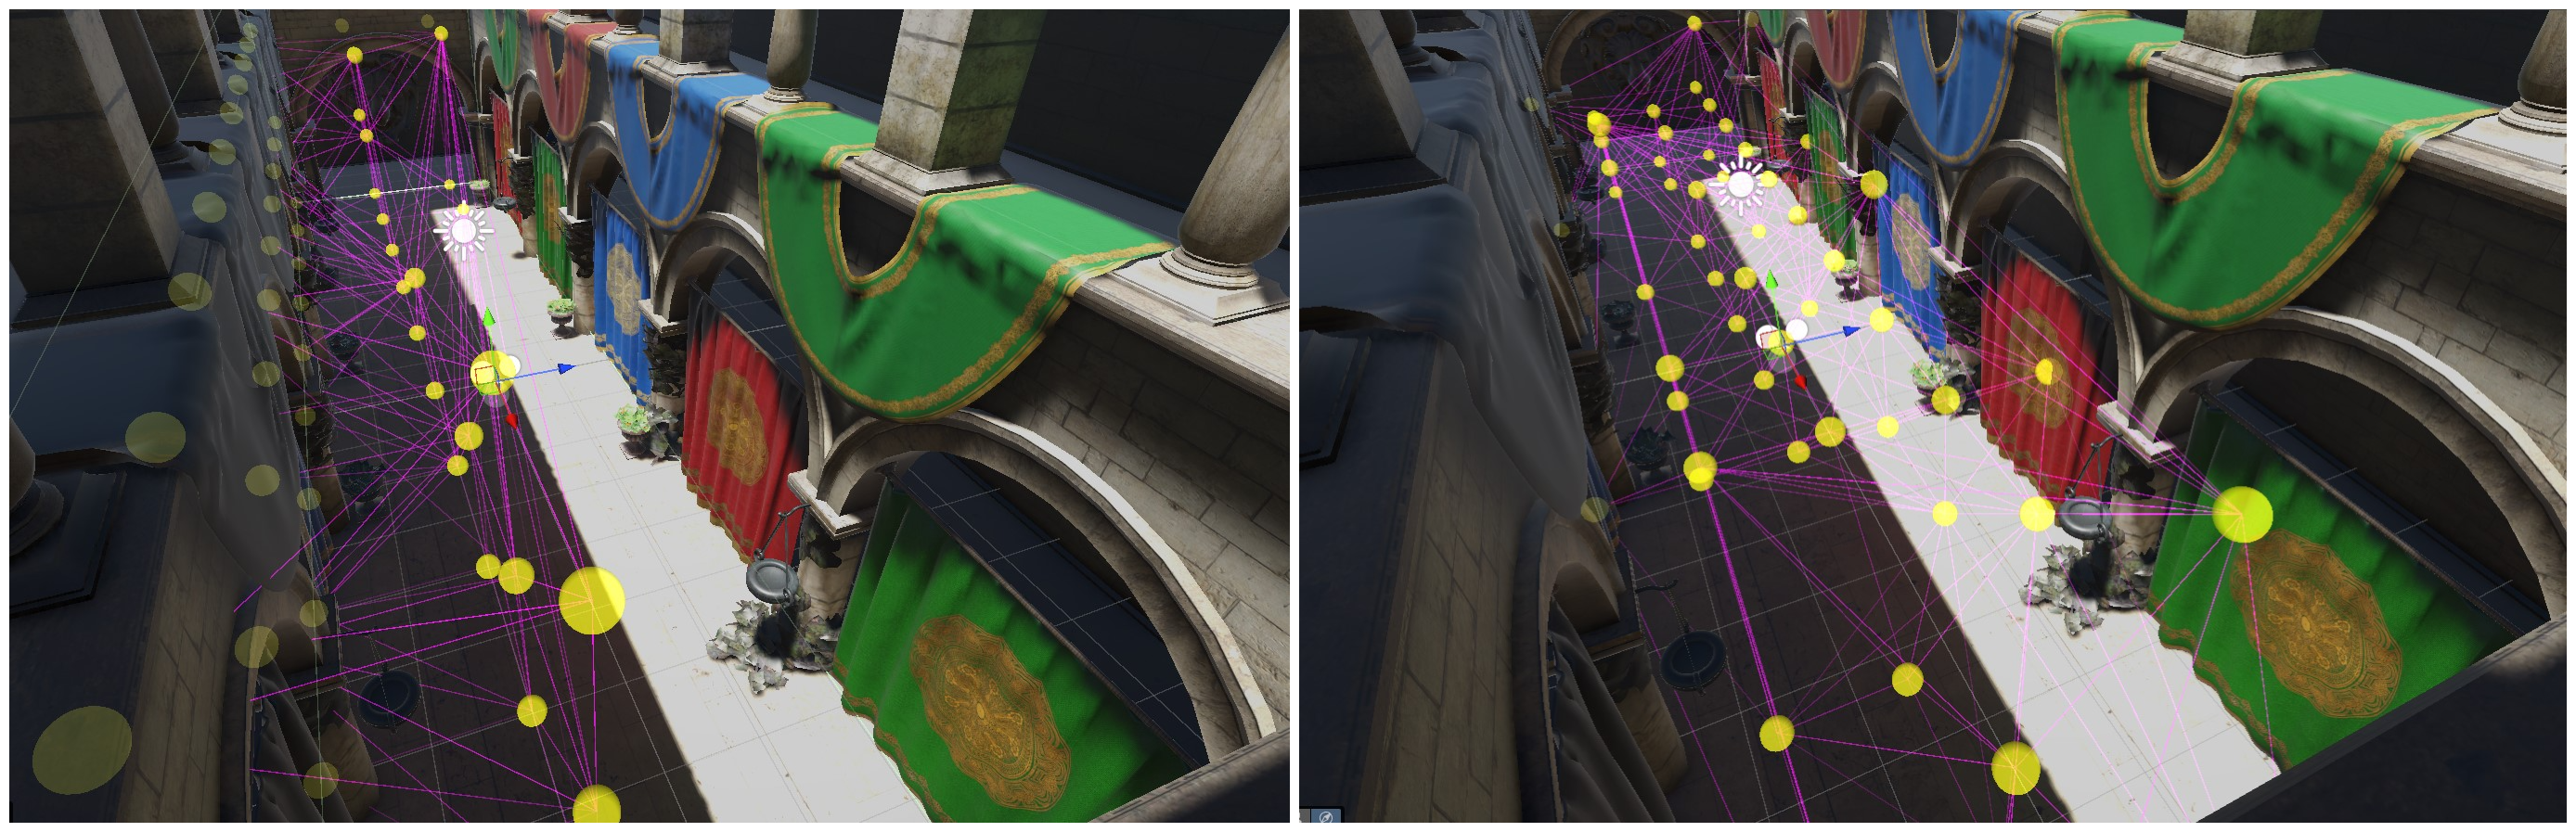
\includegraphics[width=\linewidth]{Graphics/results/concats/comparison4.png}
	\caption{A 3D Scene showing a comparison of light probe placement between LPNN (left) and LumiProbes (right) with settings 0.4, 2.0 and (12,4,5), 256 respectively, in the outdoor Sponza scene.}
	\label{fig:comp5}
\end{figure}

In figure \ref{fig:comp6} we can see the resulting layout, after manually translating the light probes a few units to the right. This process comprises of a small number of inputs required by the user, taking a few seconds to complete. The speedup of the tool is still present, even if it requires a few manual tweaks, saving time for the developer during this part of the process when developing 3D applications. In the improved layout seen in figure \ref{fig:comp6} on the right, the light probes are placed on both sides of the edge created by the angled sun illumination being occluded by the walls of the building.\newline

\begin{figure}[H]
	\centering
	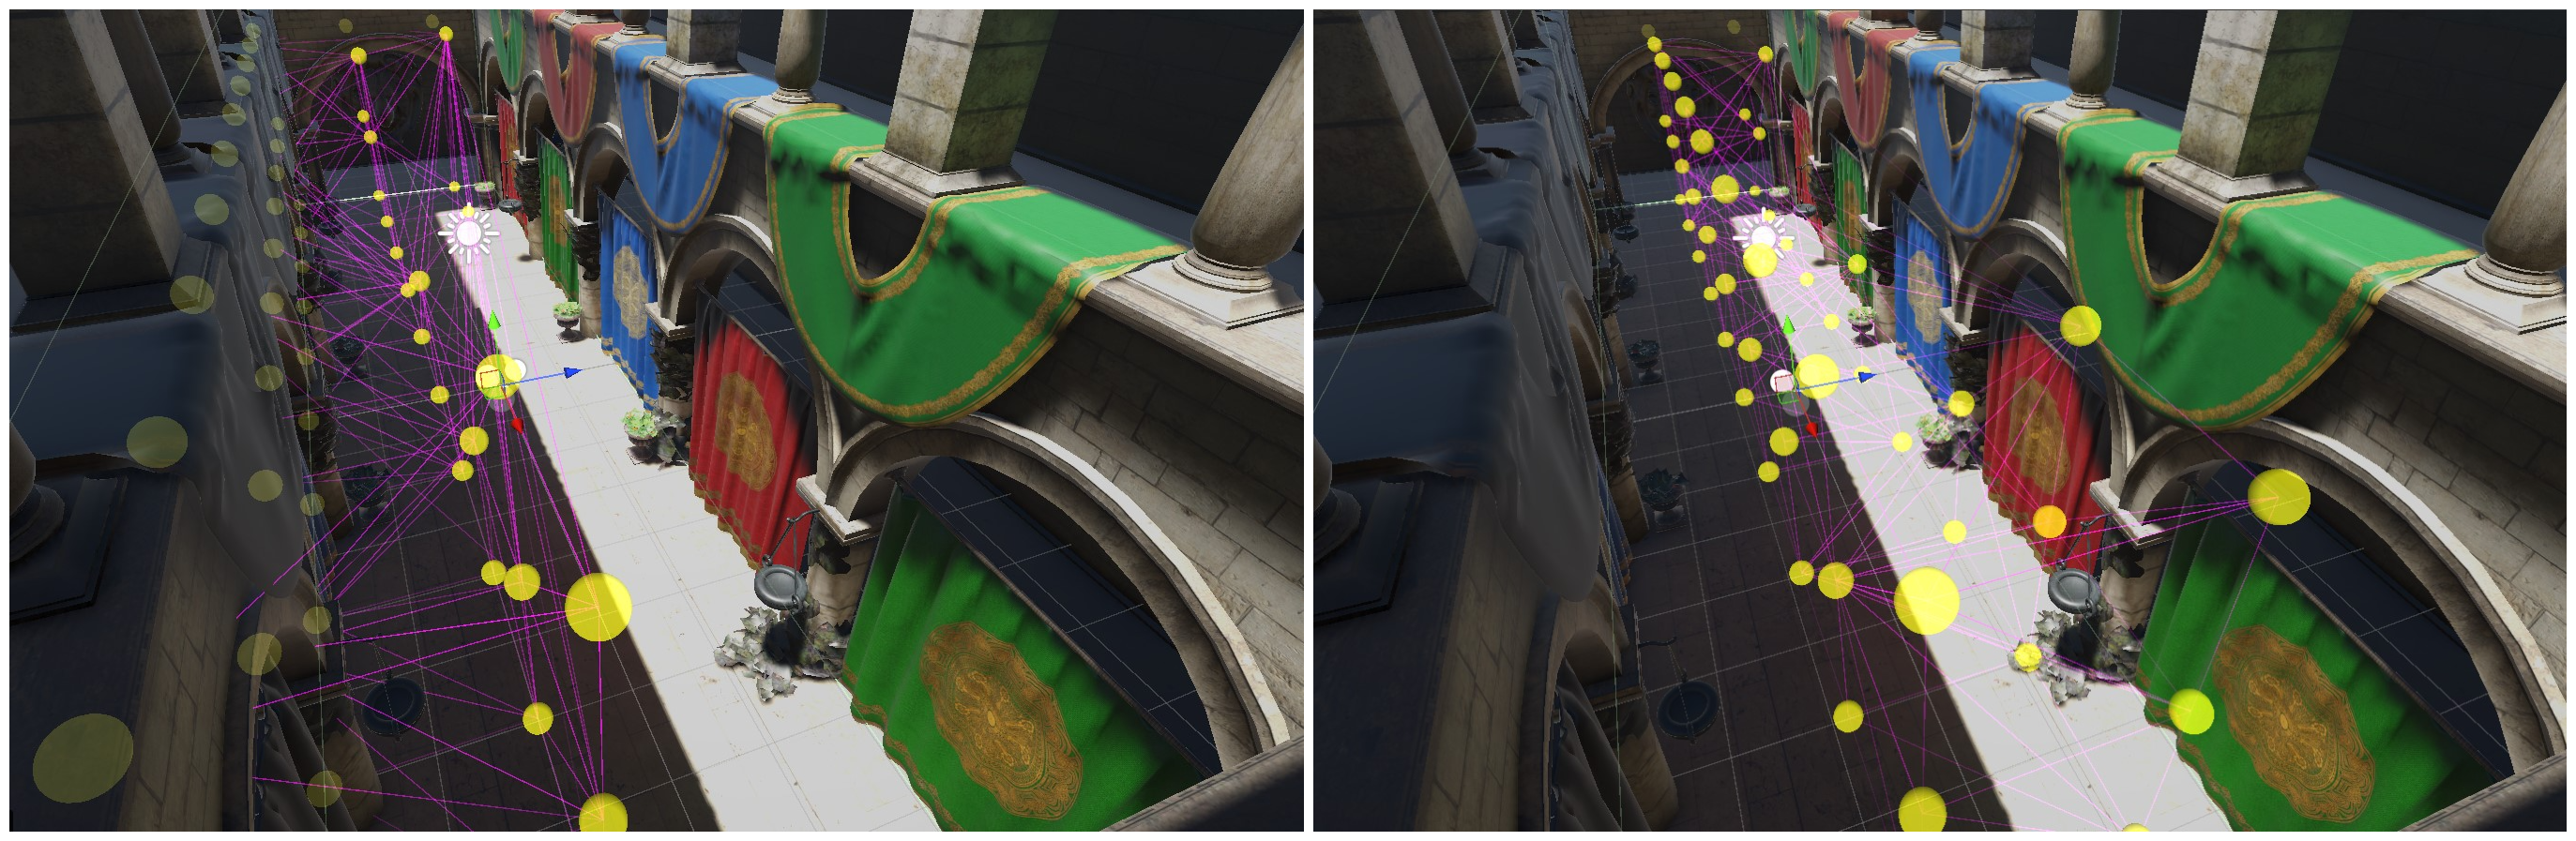
\includegraphics[width=\linewidth]{Graphics/results/concats/comparison5.png}
	\caption{A 3D Scene showing a comparison of the default light probe placement of the LPNN tool (left) and after translating the LightProbeGroup object a small number of units to the right (right).}
	\label{fig:comp6}
\end{figure}

Additionally, the tweaked layout places light probes in front of the colored surfaces on the right wall of the scene. A dynamic object that requires indirect lighting will correctly be colored lightly by the colored materials of the surfaces, and the color will also be interpolated when traversing between them. Shown closer in figure \ref{fig:sponza_detail}, we can clearly see that light probes are placed only in front of the colored materials. Taking into consideration the context of the scene, placing light probes at every grid location on that close-up area results to oversampling, placing more probes than needed, increasing the memory usage of the scene. Therefore, placing a probe between the blue and red surfaces is unnecessary, something that the LPNN model has correctly avoided. 

However, it has still dictated that a light probe between the nearby red and greed surfaces is required. With the same reasoning, we can determine that it is not vital for a light probe to be present in that location. The indirect illumination from the surfaces will be soft enough to not warrant a dense light probe layout at each location. Additionally, the edge of the shadowed area is still covered by the light probes around the mentioned position of the unnecessary light probe, since the transition between the illuminated and shadowed areas stays consistent through the scene. We decided to not manually remove the mentioned light probe for the sake of completeness, however doing so is a trivial process, comprising of only a couple of user inputs, adding only a few seconds to the total time needed for this step of the process of development.

\begin{figure}[H]
	\centering
	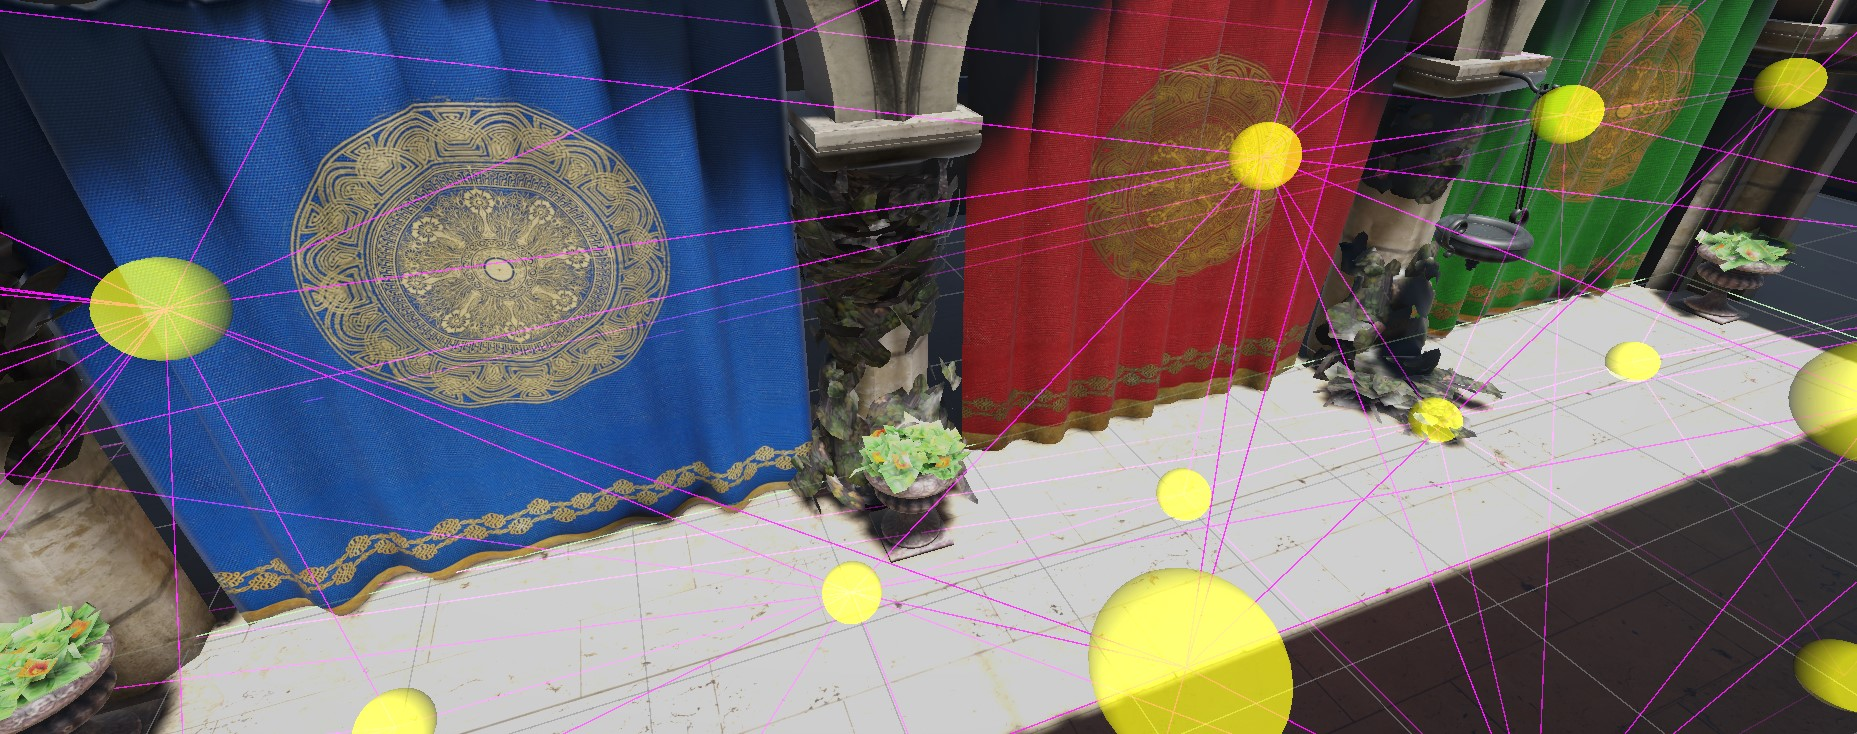
\includegraphics[width=\linewidth]{Graphics/results/sponza_0.4_2_C.jpg}
	\caption{Detailed view of the tweaked layout shown in figure \ref{fig:comp6}, showing light probes being placed in front of the colored materials, able to capture indirect illumination data for dynamic objects moving between them.}
	\label{fig:sponza_detail}
\end{figure}

Similar results were present regardless of the settings used for LPNN. The translation tool was required often, but not always. We chose to show an example using settings that best displayed our desired layout, ensuring the same number of light probes were placed with LumiProbes. The settings for both tools can be seen in the caption of figure \ref{fig:comp5}, or in table \ref{table:times}.

\subsection{Shortcomings of LPNN}

It is important to note that the light probe layout described in sub-section \ref{sec:outdoors} is inherently sub-optimal, which impacts the accuracy of dynamic object illumination. Any harsh edge in illumination, an example of which is present in the Sponza seen shown in the same sub-section, requires a tightly-packed light probe layout surrounding it, in order to ensure that a dynamic object has an instant transition between the different illuminations.

A sparser grid like the one used in the same sub-section will correctly place light probes on both sides of the light-edge, however the distance between them will make the transition smooth, resulting in inaccurate GI on the surface of a dynamic object. This issue cannot be resolved by the model, as it originates from the cell size chosen by the user, highlighting the importance of user input in achieving optimal results. Even with a theoretical perfect model, faulty user usage of the tool places the model in a state that it can only minimize the user error as best as it can. It can not resolve it, making user error one of the largest factors of sub-optimal light probe placement using the LPNN tool.\newline

\begin{figure}[h]
	\centering
	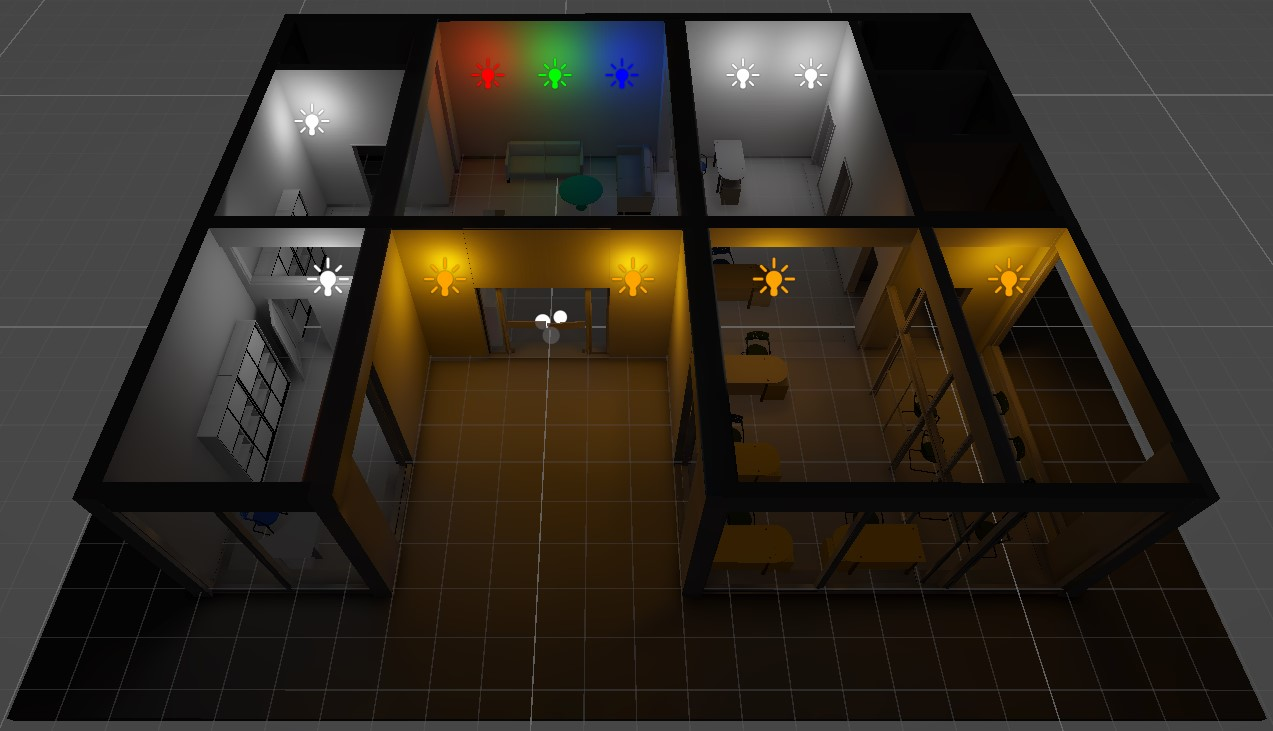
\includegraphics[width=\linewidth]{Graphics/results/office.jpg}
	\caption{The Office scene \parencite{Office2021} without any light probes placed.}
	\label{fig:office}
\end{figure}

The LPNN model used during the creation of this thesis can be improved. In rare occasions, the inferred importance scores fail to cover areas of high GI variance. As seen in figure \ref{fig:office_faulty}, the light probes placed by LPNN (left) fail to completely capture the lighting information of the three colored light sources in one room. Additionally, no light probes were placed in the left of the scene, near the white light source. Any dynamic object in this scene will receive insufficient illumination data, resulting in incorrect surface color.\newline

\begin{figure}[h]
	\centering
	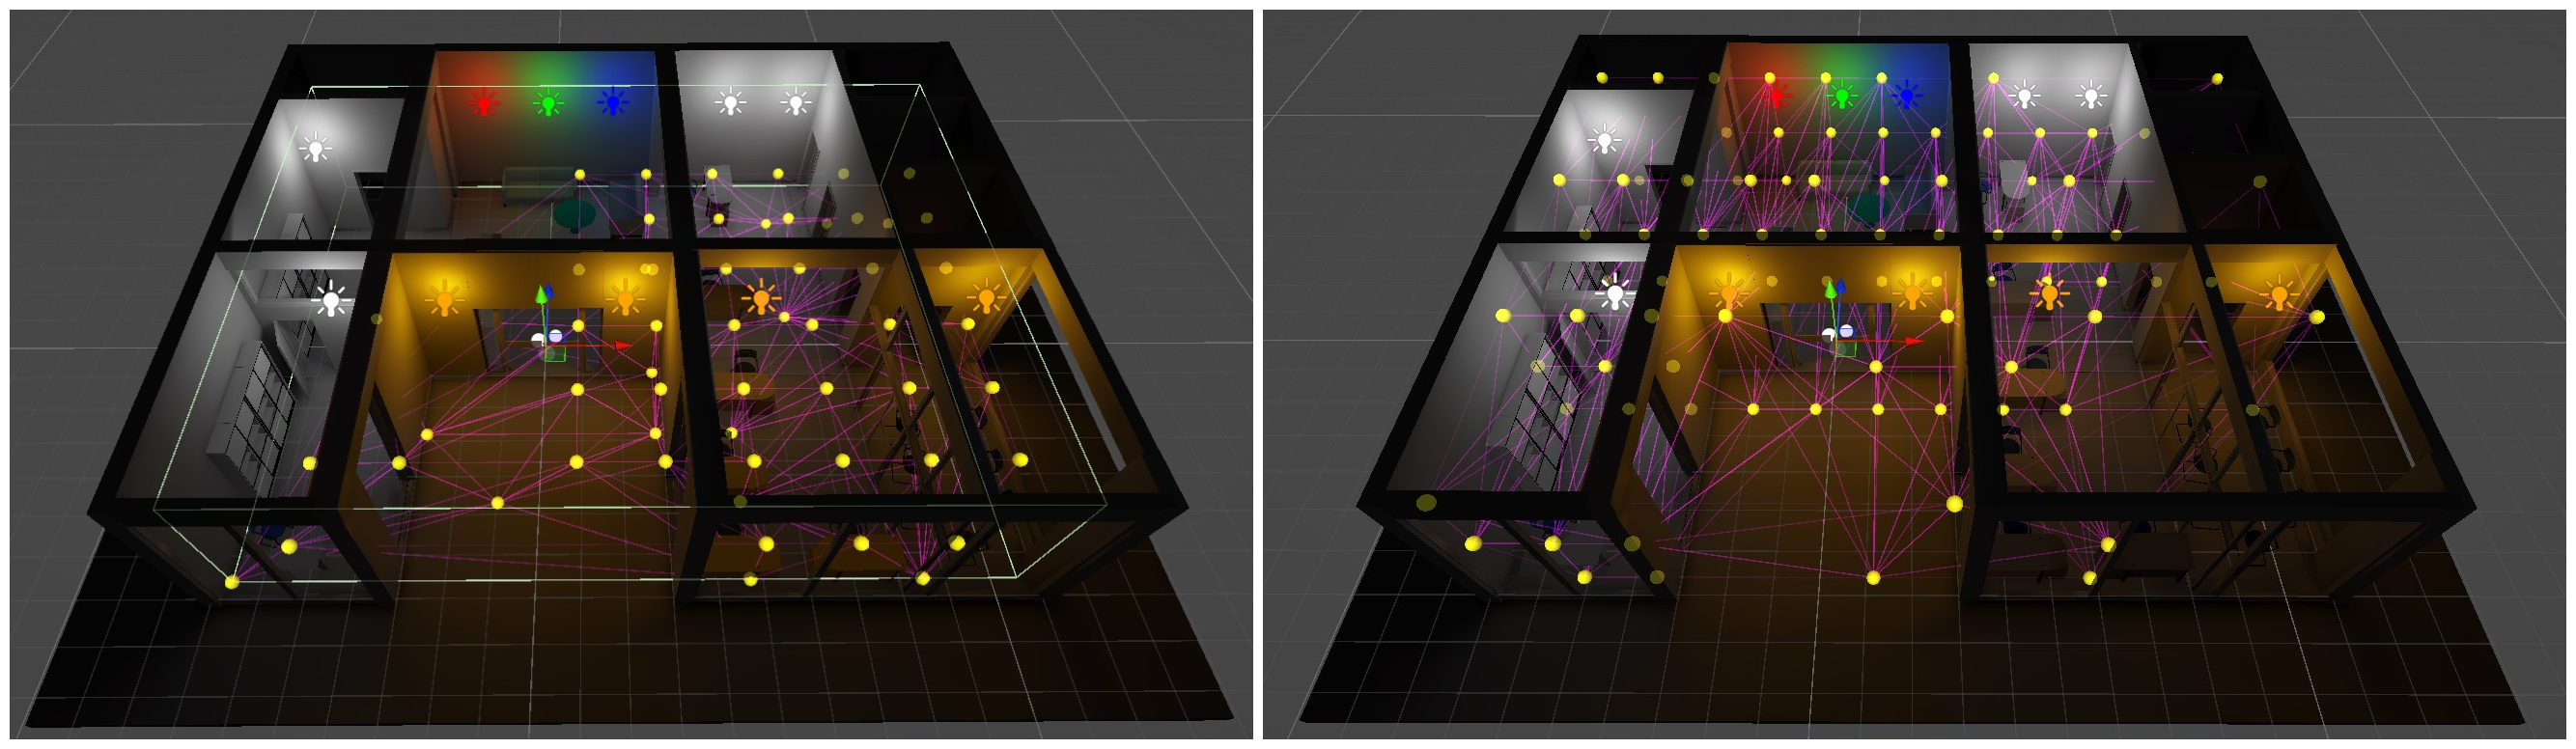
\includegraphics[width=\linewidth]{Graphics/results/concats/comparison6.png}
	\caption{Overview of faulty light probe placement inferred by the model. Settings used are 0.758, 1.87 for LPNN (left) and (12,3,4), 128 for LumiProbes (right).}
	\label{fig:office_faulty}
\end{figure}

Additionally, in the same scene, we can see that the right half of the building contains multiple light probes, even in areas where the change in illumination is minimal or non-existent. Not all light probes are unnecessary. A dynamic object in this part of the scene will have sufficient data from the light probes surrounding it, therefore the surface of the object will be shaded correctly. However, due to the lack of significant illumination changes, the amount of placed light probes can be reduced significantly, while keeping the same visual quality. The currently oversampled area results in increased memory usage with no improvements in the quality of GI on dynamic objects.\newline

This problem results from the model itself. It is important to have sufficient amount of high quality data during training; data from a variety of scenes and examples, including many edge-cases and variations. We trained the model using 3485 total feature vectors from different scenes, as detailed in section \ref{sec:model_training}. However, a bigger dataset can improve the accuracy of the model, potentially avoiding the issue mentioned. In cases like the one described, it is necessary that the user attempts using different settings for the tool and potentially requiring an increased manual tweaking process to provide the desired results.

With different settings, mainly a much denser EP grid, the importance scores inferred by the model improve slightly. Even though they are still suboptimal, the light probes are located in areas of variance more often, but still failing to appear in all and with proper layout. As seen in figure \ref{fig:office_faulty_new}, the model successfully placed light probes around the three differently-colored light sources in the central room, and additionally placed probes on the white light source to the left of the room. Furthermore, a few light probes were placed on the dark rooms on the two corners of the building, ensuring a dynamic object will be properly shaded when entering those areas.

\begin{figure}[h]
	\centering
	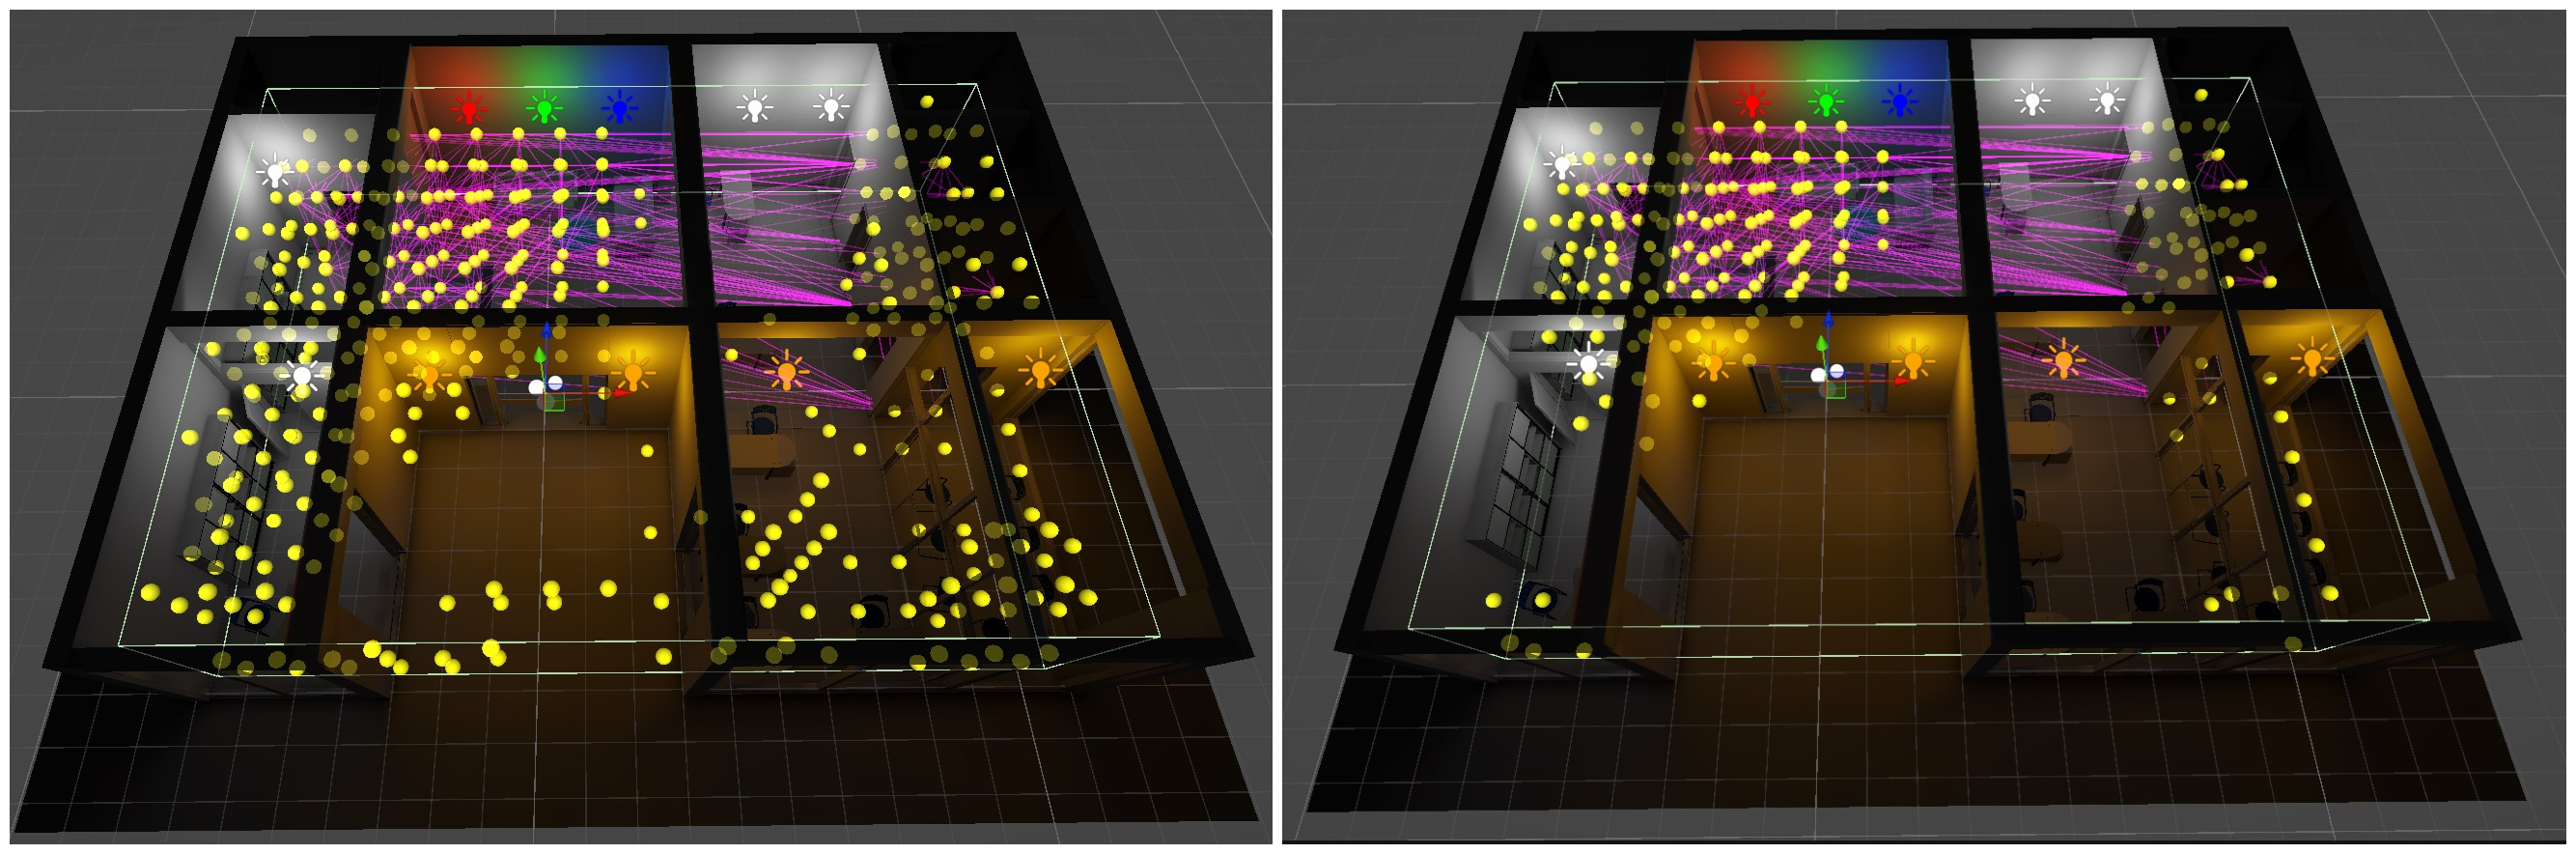
\includegraphics[width=\linewidth]{Graphics/results/concats/comparison9.png}
	\caption{Overview of faulty light probe placement inferred by the model. Settings used are 0.611, 1 (left) and 0.785, 1 (right), done in the Office scene.}
	\label{fig:office_faulty_new}
\end{figure}

However, it is apparent that this layout is still not sufficient. The large amount of light probes placed, even with an increased threshold, as seen in the same figure \ref{fig:office_faulty_new}, results in much higher memory usage during runtime, greatly impacting the performance of the application. Furthermore, in an attempt to reduce the number of light probes by increasing the threshold, keeping only the most important light probes, we can see a significant gap in light probe placement in areas of high variance. Namely, on the image on the right of figure \ref{fig:office_faulty_new}, the rooms on the bottom of the figure, as well as the room with the two white light sources lack significantly in light probe coverage. Any dynamic object traversing those rooms will receive incorrect lighting, immediately visible to the user. 

Furthermore, the dense grid and consequently the large amount of light probes placed makes manual tweaking by the developer a very time-consuming task. It is natural for the developer to require the most optimal layout for the present scene, but relocating each light probe in this current scenario will take approximately the same amount of time than placing the light probes manually.\newline

\begin{figure}[h]
	\centering
	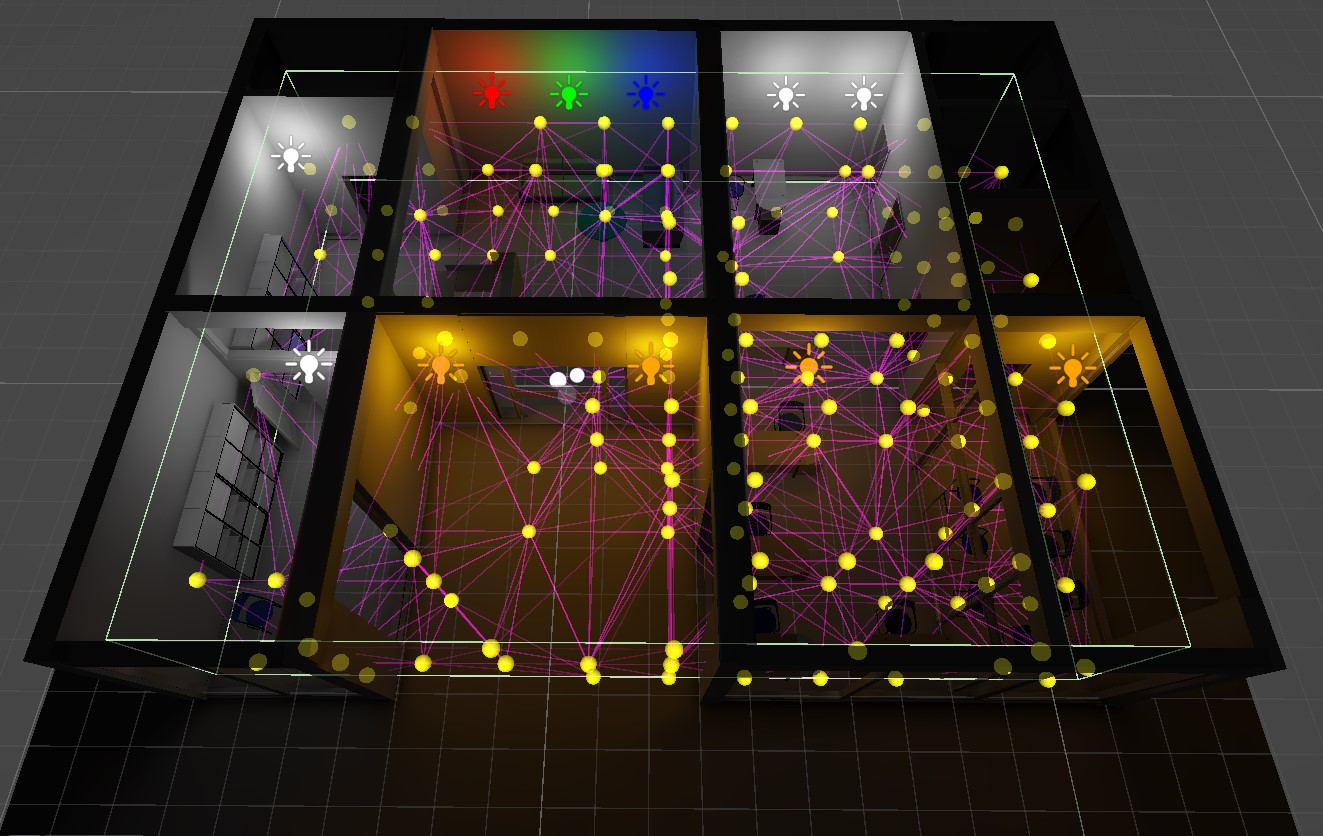
\includegraphics[width=\linewidth]{Graphics/results/office_0.35_1.49.jpg}
	\caption{Overview of an improved light probe placement inferred by the model. Small manual tweaking was done to remove a small number of light probes. Settings used are 0.35, 1.49 in the Office scene.}
	\label{fig:office_faulty_better}
\end{figure}

Even though the two examples shown in figures \ref{fig:office_faulty} and \ref{fig:office_faulty_new} are from the same scene, with the only difference being the size of the cell which results in a denser grid, the innate uncertainty of a Neural Network model results in an inferred output that can on occasion be faulty or incorrect, as presented. Additional tweaking of the cell size and the threshold value can create an improved layout for the light probes, as seen in figure \ref{fig:office_faulty_better}. 

The new layout has placed more light probes on the areas mentioned before, specifically those that contained minimal or none at all. The rooms on the right of the building have enough light probes to capture the transition between the colored lights and the white lights, the orange lights and the white lights as well as the white light sources and the dark rooms on the right corner of the building. This resolves most issues with the previous layout, as well as reducing the density of the grid and therefore the amount of light probes present in the scene.

However, it is important to mention that the layout present in figure \ref{fig:office_faulty_better} has been tweaked manually, and is not the default result inferred by the LPNN model with the setting specified in the caption of the figure. We manually tweaked the layout by removing a small number of light probes from densely populated areas, since their impact to the accuracy of lighting information on a dynamic object is not vital. No other manual tweaking was done; the positions of light probes that were not removed is the same, and no light probes were added to the grid and placed manually. The manual process was completed within 5 minutes from the moment the model placed the initial layout of light probes with the provided settings. In total, from the moment we first opened the scene in Unity to the moment of capturing the result, the time spent was close to 10 minutes of real time. Even though manually placing the light probes is a process that requires much more time, especially on larger scenes, the results present can still be improved upon to approach the theoretical optimal even more.

We can clearly see that the process of finding the best layout by experimenting with the settings is a process that can on occasion result to sub-optimal light probe layouts, requiring manual tweaking or ,on rare occasions, even restart of the process. Work can be done to improve the model and the tool, as described in section \ref{sec:Conclusions}.